\chapter{Limitations and Discussion}\label{chap:discussion}
\subsection{Future Work}
Due to time contraints on the project, not all the cases in \autoref{tab:combos} were tested. Only the three selected baseline poses shown in \autoref{fig:bpose1}, \autoref{fig:bpose2}, and \autoref{fig:bpose3} were ever considered in practice. The algorithm described in the report to merge hierarchies assumes that the characters being merged are already in the desired position for connection. This means that if the user wanted the characters to be holding hands -- a contact to be maintained -- the hands should be already touching when the user selects and merges joints. Ideally, the user should be able to specify whether or not they want a merge to create a contact. Currently, if they do want a contact, the hands in this example should move to be touching. If not, the combined node's averaged frame will be somewhere in between the two hands, whether they are close in position or not. This could possibly be solved with a better joint selection method.

\subsection{Joint Selection}
The joint selection interface idea was originally to have the user encircle the joints they want to be merged. This comes with problems and advantages, the benefit being that it may be more intuitive to the user. However, a method for detecting all joints in the 2D circle would be challenging. Along with that difficulty, there would be some ambiguity as to which joints the user actually wants in their circle. Some joints will be behind others in the 3D space and who is to say whether those unseen joints should or should not be included in the selection?

To that effect, currently only pairs of joints can be selected and merged. It could be interesting to see what changes, if any, would be needed for the merging algorithm if the user were allowed to select an arbitrary number of joints. There is more potential for creating cycles that way, which would make very large combined nodes. On the one hand, less computation would be required in the body line selection and posing because there are fewer joints to choose from in the merged hierarchy. But on the other hand, the resulting rigid body made of nodes could gradually increase to be bigger than the user intended and makes for a less precise pose.

\subsection{User Constraints}
Users are only allowed to attach and detach hierarchies at keyframes to avoid interpolation issues. If a contact made by the merged hierarchy is present in one keyframe and absent in the next, the splitting of the hierarchy would have to be done during the interpolation at some time in between the two keyframes. So for now the user can only make sets of keyframes where the actual detaching is done exactly at a keyframe.

\subsection{Taking Advantage of Patterns}
Symmetry and parallelism are both prevalent in the use case video. It would be nice to use this to make posing even faster. For example, while posing one character, the system could pose the other in the same or opposite way. This would involve mirroring the drawn LOA to match to the second characters, limb. This raises questions about which kinematic chain on the second character to select. 

\begin{figure}[h!]
	\centering
        \begin{subfigure}[b!]{0.45\textwidth}
        	\centering
                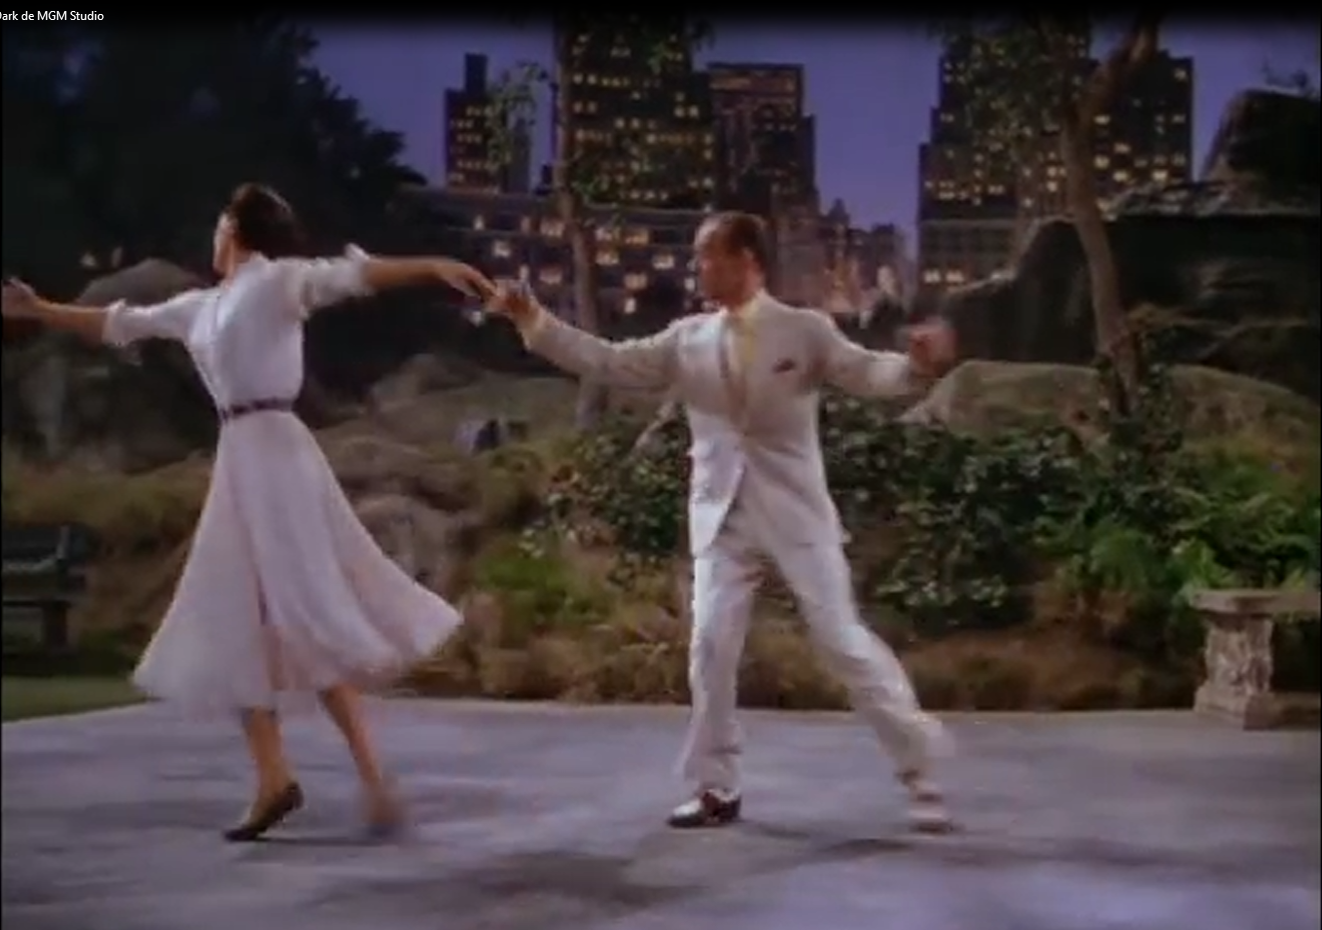
\includegraphics[width=\linewidth]{img/parallelism}
                \caption{Parallelism.}
                \label{fig:parallelism}
        \end{subfigure}
        \quad
        \begin{subfigure}[b!]{0.45\textwidth}
        	\centering
                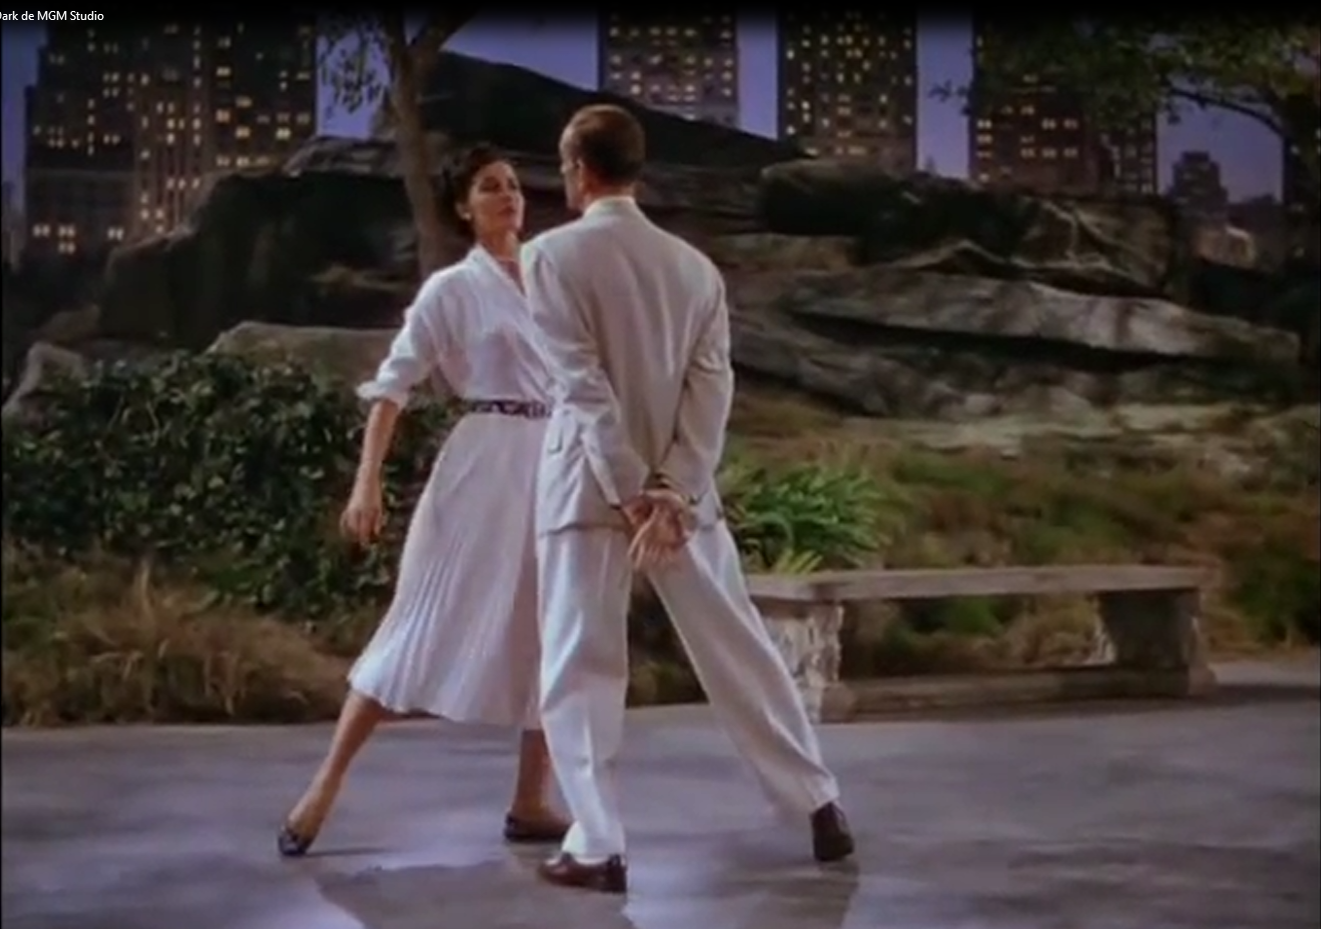
\includegraphics[width=\linewidth]{img/symmetry}
                \caption{Symmetry.}
                \label{fig:symmetry}
        \end{subfigure}%
        \caption{Patterns in the poses.}
	\label{fig:patterns}
\end{figure}

\subsection{Twisting}
In future work, the twisting problem mentioned in \autoref{chap:issues} would be very nice to explore, since the amount of spins the dancing characters do is quite high. The characters spin separately and together, so the technique would need to work on both separate and combined kinematic trees.
\begin{figure}[!h]
\centering
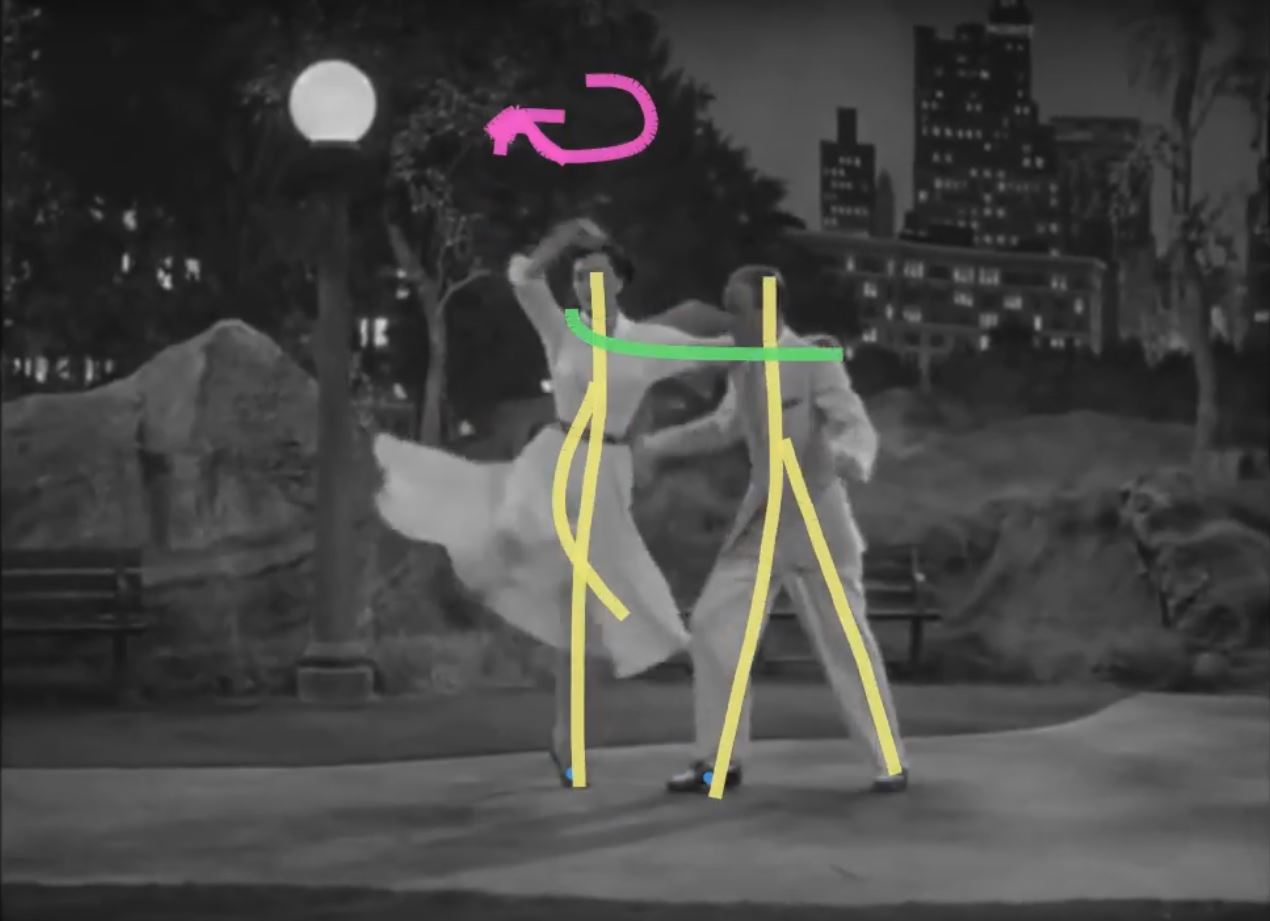
\includegraphics[scale=0.5]{img/twistingannotation}
\caption{One idea for a twisting notation.}
\end{figure}